
\begin{center}\texttt{1 - Lifecycle and Developement Processes}\end{center}
\hrulefill \\
Life Cycle refers to the states that a given entity can assume during
the span of its life: for a software product, a life cycle could go from an init phase (rough idea) to the product retirement, passing through development, release, support.

 Software development process relates to strategies to be adopted to
manage the life cycle of a software product. In particular, it identifies
when and who should do what to reach a given objective in the
management of the life-cycle. It's a set of activities, basically.

 Macro-activities of some process typically include:
\begin{itemize}
    \item communication (define specs and requirements). Requirements engineering consists of:
    \begin{itemize}
        \item feasibility study;
        \item req elicitation and analysis;
        \item req specification;
        \item req validation (realistic, complete...);
    \end{itemize}
    \item planning (risks and costs);
    \item design (models, e.g. UML diagrams or agile methodologies);
    \item construction (implementation and verification);
    \item deployment.
\end{itemize}

 ``Planning is useful, plan is useless'': planning is about exploring possibilities and deciding to pursue one based on whatever criterion; plans are useless means that reality is often different from the scenario considered during planning, things often go unexpected ways therefore the plan we had ends up being inadequate in the end. Still, planning activities are the ones that prove insightful so are generally recommended.

Phases are periods of time during which we want to reach some objectives ($\approx$ artefacts) - different phase, different activities, different objectives. In the Waterfall model, Phases and Activities correspond $1:1$, but that is not always the case (E.g.: UP).\\
\noindent \underline{The Waterfall Model}\\
Old classic model which is not iterative: each activity is ``definitive'' and is never revisited - though two activities might overlap to guarantee better flow of information (i.e. one begins before the previous one is considered finished). With this model it is especially important to have a clear, complete and definitive Requirements document. A lot of time is thus invested in the Requirements definition phase in the waterfall model.
\begin{figure} [H]
    \centering
    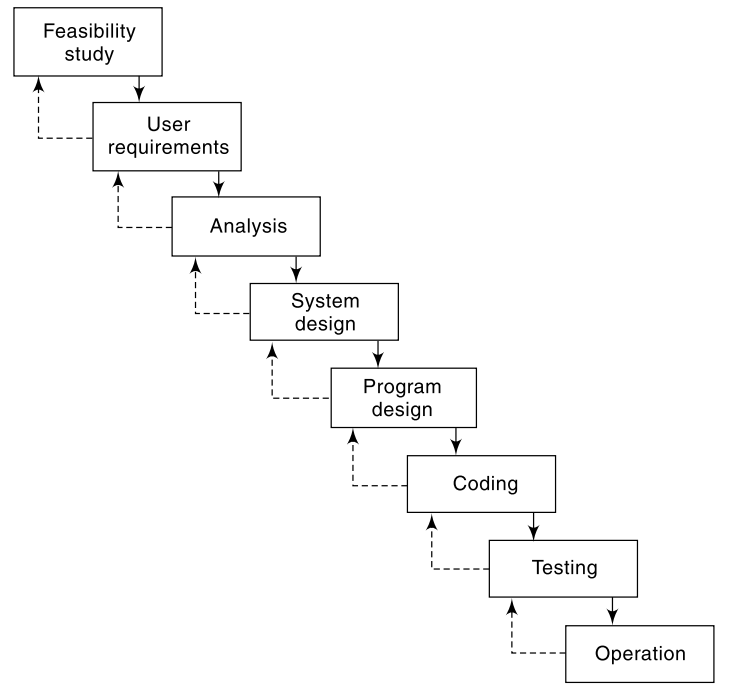
\includegraphics[scale=0.4]{Figures/01/waterfall00.png}
    \caption{The Waterfall Model (Cotterell-Hughes 2011)}
    \label{fig:wf1}
\end{figure}

Because of its definition, the process becomes unresponsive to request of requirements modification; it produces strongly documented software and document driven development (unlike Agile methodologies);

\noindent [Note from C-H11]: The waterfall approach may be favoured by some managements because it creates natural milestones at the end of each phase. At these points, managers can review project progress to see whether the business case for the project is still valid.

\noindent \underline{Spiral Model}\\
\noindent I.e., another way of looking at the waterfall model. Characteristic features of the spiral model are the incremental style of development and the ability to handle various types of risks. Each loop of the spiral is called a phase of this software process. In each phase, one or more features of the product are implemented after resolving any associated risks through 
prototyping.

 \noindent Prototyping: dev technique, consists in developing incremental versions of the product, e.g.: by increasingly adding demonstrable features (evolutionary prototyping). Supports communication and customer interaction, allows to clarify requirements in-itinere, reduces need for documentation; however, it can be difficult to control and cover cost-wise, might open to inefficiency with hardware and sloppy features.

\noindent Prototyping is usually done only to some extent: for example, interfaces and functionalities can be prototyped through mockups, simulated interactions and partial simulations that can be approximated horizontally or vertically.

\begin{figure} [H]
    \centering
    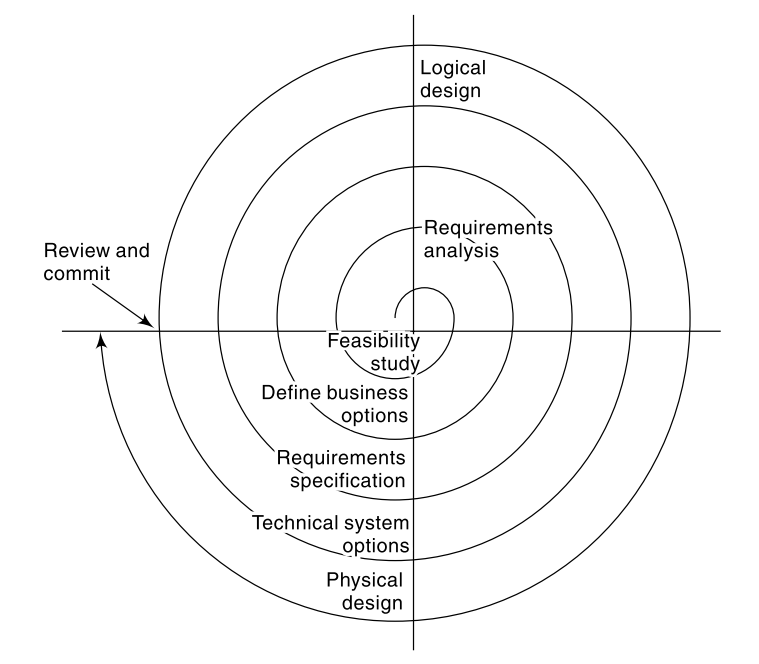
\includegraphics[scale=0.4]{Figures/01/spiral00.png}
    \caption{The Spiral Model (Cotterell-Hughes 2011)}
    \label{fig:sm1}
\end{figure}

\noindent \underline{Iterative Models}\\
\noindent Based on the concept of iteration (the specification evolves together with the system development): each iteration is a stand-alone little waterfall and the process is overall incremental, i.e. it leads to the delivery of a working system that the customer can try out, each time with new features. Allows to test important features more exhaustively, improves customer interaction, especially suitable for teams of small size.

 Brief overview of the UP: risk-driven \& driven by Use Cases (please remember this by yourself lol), incremental, iterative. Each iteration consists of a sequence of activities:
 \begin{itemize}
     \item planning;
     \item requirements;
     \item analysis;
     \item design;
     \item development;
     \item test \& integration;
     \item validation \& release.
 \end{itemize}
The life-cycle is divided in 4 phases: inception, elaboration, construction, and transition. Each iteration ends with a baseline, i.e. the set of artefacts revised and approved (codebase, documents, etc.). You will start from this baseline in the next iteration to generate an increment. Each phase ends with a milestone (I guess a big goal in artefacts and stuff).

 